\documentclass[aspectratio=169,10pt]{beamer}
\usetheme{Madrid}
\usepackage[T1]{fontenc}
\usepackage{lmodern}
\usepackage{tikz}
\usepackage{adjustbox}
\usepackage{tcolorbox}
\tcbuselibrary{skins}
\usepackage{fontawesome5}
\usetikzlibrary{arrows.meta,positioning,fit,backgrounds,calc,shadows,shapes.geometric}

\definecolor{prismNavy}{RGB}{11,31,58}
\definecolor{prismBlue}{RGB}{0,168,198}
\definecolor{prismTeal}{RGB}{22,138,114}
\definecolor{prismMint}{RGB}{221,244,247}
\definecolor{prismGold}{RGB}{217,154,34}
\definecolor{prismDark}{RGB}{23,32,42}
\definecolor{prismLight}{RGB}{244,248,251}
\definecolor{prismIndigo}{RGB}{23,54,93}
\definecolor{prismSlate}{RGB}{102,112,133}

\definecolor{lavenderDark}{RGB}{75,45,115}
\definecolor{lavenderMedium}{RGB}{140,110,180}
\definecolor{lavenderLight}{RGB}{235,230,248}

\definecolor{cInput}{RGB}{231,233,236}
\definecolor{cStem}{RGB}{220,214,247}
\definecolor{cPlanner}{RGB}{207,199,242}
\definecolor{cDispatch}{RGB}{169,220,235}
\definecolor{cMemory}{RGB}{214,185,230}
\definecolor{cReact}{RGB}{169,222,200}
\definecolor{cTool}{RGB}{244,213,141}
\definecolor{cDeliverable}{RGB}{185,222,210}
\definecolor{cSafety}{RGB}{240,170,167}
\definecolor{cOutput}{RGB}{234,207,213}
\definecolor{cBadge}{RGB}{255,255,255}

\setbeamercolor{frametitle}{bg=lavenderDark,fg=white}
\setbeamercolor{background canvas}{bg=white}
\setbeamertemplate{navigation symbols}{}

\begin{document}

% =============================================================================
% SLIDE 09: SYSTEM ARCHITECTURE & 11-MODEL CONNECTIONS (FIGURE 1.2)
% =============================================================================
\begin{frame}[t]{09. PrismSpace System Architecture \& Multi-Model Swarm Workflow (Figure 1.2)}
\vspace{-0.32em}
\centering
\adjustbox{max width=0.96\linewidth, max height=0.69\textheight}{%
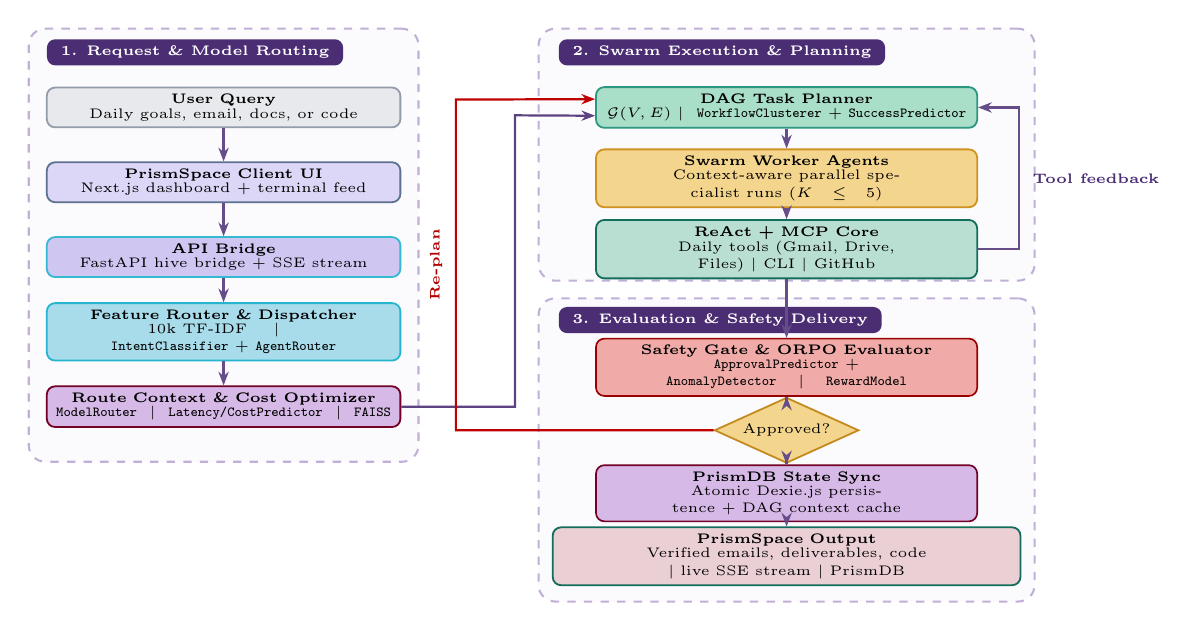
\begin{tikzpicture}[
  x=1cm, y=1cm,
  every node/.style={align=center},
  group/.style={draw=lavenderMedium!55, dashed, line width=0.75pt,
    fill=lavenderLight!22, rounded corners=6pt},
  grouptitle/.style={fill=lavenderDark, text=white, font=\fontsize{5.2}{6.2}\selectfont\bfseries,
    rounded corners=3pt, inner xsep=5pt, inner ysep=2.5pt},
  flowbox/.style={rectangle, rounded corners=3pt, line width=0.65pt,
    text width=4.35cm, minimum height=0.50cm, inner ysep=2.4pt, inner xsep=2pt,
    font=\fontsize{5.2}{6.2}\selectfont},
  smallbox/.style={rectangle, rounded corners=3pt, line width=0.6pt,
    text width=4.35cm, minimum height=0.50cm, inner ysep=2.4pt, inner xsep=2pt,
    font=\fontsize{5.1}{6.1}\selectfont},
  decision/.style={diamond, aspect=2.2, draw=prismGold!90!black,
    fill=cTool, line width=0.65pt, inner xsep=2pt, inner ysep=1.5pt,
    font=\fontsize{5.2}{6.2}\selectfont},
  arrow/.style={
    -{Stealth[scale=0.75]}, line width=0.8pt, draw=lavenderDark!85
  }
]

  % 1. INPUT & ORCHESTRATION
  \node[group, minimum width=4.95cm, minimum height=5.5cm] (g1) at (2.50, 3.50) {};
  \node[grouptitle, anchor=west] at (0.25, 5.95) {1. Request \& Model Routing};
  \node[flowbox, fill=cInput, draw=prismSlate!70] (start) at (2.50, 5.25) {\textbf{User Query}\\[-0.15em] Daily goals, email, docs, or code};
  \node[flowbox, fill=cStem, draw=prismIndigo!70] (intent) at (2.50, 4.30) {\textbf{PrismSpace Client UI}\\[-0.15em] Next.js dashboard + terminal feed};
  \node[flowbox, fill=cPlanner, draw=prismBlue!80] (plan) at (2.50, 3.35) {\textbf{API Bridge}\\[-0.15em] FastAPI hive bridge + SSE stream};
  \node[flowbox, fill=cDispatch, draw=prismBlue!85] (dispatch) at (2.50, 2.40) {%
    \textbf{Feature Router \& Dispatcher}\\[-0.15em]
    10k TF-IDF $\;\vert\;$ \textbf{\texttt{IntentClassifier}} + \textbf{\texttt{AgentRouter}}%
  };
  \node[flowbox, fill=cMemory, draw=purple!60!black] (state) at (2.50, 1.45) {%
    \textbf{Route Context \& Cost Optimizer}\\[-0.15em]
    \textbf{\texttt{ModelRouter}} $\;\vert\;$ \textbf{\texttt{Latency/CostPredictor}} $\;\vert\;$ \textbf{\texttt{FAISS}}%
  };
  \draw[arrow] (start)--(intent); \draw[arrow] (intent)--(plan); \draw[arrow] (plan)--(dispatch); \draw[arrow] (dispatch)--(state);

  % 2. EXECUTION & TOOLS
  \node[group, minimum width=6.3cm, minimum height=3.2cm] (g2) at (9.65, 4.65) {};
  \node[grouptitle, anchor=west] at (6.75, 5.95) {2. Swarm Execution \& Planning};
  \node[flowbox, text width=4.7cm, fill=cReact, draw=prismTeal!90] (react) at (9.65, 5.25) {%
    \textbf{DAG Task Planner}\\[-0.15em]
    $\mathcal{G}(V,E) \;\vert\;$ \textbf{\texttt{WorkflowClusterer}} + \textbf{\texttt{SuccessPredictor}}%
  };
  \node[flowbox, text width=4.7cm, fill=cTool, draw=prismGold!95!black] (mcp) at (9.65, 4.35) {%
    \textbf{Swarm Worker Agents}\\[-0.15em]
    Context-aware parallel specialist runs ($K \le 5$)%
  };
  \node[flowbox, text width=4.7cm, fill=cDeliverable, draw=prismTeal!80!black] (result) at (9.65, 3.45) {%
    \textbf{ReAct + MCP Core}\\[-0.15em]
    Daily tools (Gmail, Drive, Files) $\vert$ CLI $\vert$ GitHub%
  };
  \draw[arrow] (react)--(mcp); \draw[arrow] (mcp)--(result);
  \draw[arrow] (result.east) -- (12.60, 3.45) -- (12.60, 5.25) -- (react.east);
  \node[font=\fontsize{5}{6}\selectfont\bfseries, text=lavenderDark, anchor=west] at (12.65, 4.35) {Tool feedback};

  % 3. VERIFICATION & OUTPUT
  \node[group, minimum width=6.3cm, minimum height=3.85cm] (g3) at (9.65, 0.90) {};
  \node[grouptitle, anchor=west] at (6.75, 2.55) {3. Evaluation \& Safety Delivery};
  \node[smallbox, text width=4.7cm, fill=cSafety, draw=red!60!black] (verify) at (9.65, 1.95) {%
    \textbf{Safety Gate \& ORPO Evaluator}\\[-0.15em]
    \textbf{\texttt{ApprovalPredictor}} + \textbf{\texttt{AnomalyDetector}} $\;\vert\;$ \textbf{\texttt{RewardModel}}%
  };
  \node[decision] (pass) at (9.65, 1.15) {Approved?};
  \node[smallbox, text width=4.7cm, fill=cMemory, draw=purple!60!black] (synth) at (9.65, 0.35) {%
    \textbf{PrismDB State Sync}\\[-0.15em]
    Atomic Dexie.js persistence + DAG context cache%
  };
  \node[flowbox, text width=5.8cm, fill=cOutput, draw=prismTeal!80!black] (out) at (9.65, -0.45) {%
    \textbf{PrismSpace Output}\\[-0.15em]
    Verified emails, deliverables, code $\vert$ live SSE stream $\vert$ PrismDB%
  };

  % Connecting result to verify (stage 2 to stage 3)
  \draw[arrow] (result.south) -- (verify.north);
  \draw[arrow] (verify) -- (pass);
  \draw[arrow] (pass) -- (synth);
  \draw[arrow] (synth) -- (out);

  % Inter-group routing lines in channel between g1 and g2/g3
  % Rail 1 (Route Context -> DAG Task Planner) at x=6.20 (Inner Rail)
  \draw[arrow, draw=lavenderDark!90, line width=0.8pt] (state.east) -- (6.20, 1.45) -- (6.20, 5.15) -- ([yshift=-3pt]react.west);

  % Rail 2 (Re-plan feedback from Approved?) at x=5.45 (Outer Rail)
  \draw[arrow, draw=red!75!black, line width=0.8pt] (pass.west) -- (5.45, 1.15) -- (5.45, 5.35) -- ([yshift=3pt]react.west);
  \node[font=\fontsize{5}{6}\selectfont\bfseries, text=red!70!black, rotate=90] at (5.20, 3.25) {Re-plan};

\end{tikzpicture}%
}
\vspace{-0.22cm}
\begin{tcolorbox}[
  width=0.99\linewidth, enhanced, arc=3pt,
  colframe=lavenderDark!65, colback=lavenderLight!35, boxrule=0.6pt,
  left=3pt, right=3pt, top=1.2pt, bottom=1.2pt
]
\centering
{\fontsize{4.1}{4.9}\selectfont\color{lavenderDark}
\textbf{11 Models Mapped from \texttt{Models/}:}
\textbf{Stage 1:} \texttt{intent\_classifier} (12-class), \texttt{agent\_router} (specialist team), \texttt{model\_router} (OpenAI/Groq/NIM), \texttt{latency\_predictor}, \texttt{cost\_predictor}, \texttt{faiss.index} (semantic ranker) $\;\vert\;$
\textbf{Stage 2:} \texttt{workflow\_templates} (clusterer), \texttt{workflow\_success\_predictor} (DAG completion) $\;\vert\;$
\textbf{Stage 3:} \texttt{approval\_predictor} (risk score), \texttt{anomaly\_detector} (IsolationForest), \texttt{reward\_orpo\_v2} (TRL Odds Ratio Alignment)
}
\end{tcolorbox}
\end{frame}


% =============================================================================
% SLIDE 10: UNIFIED DATASET PREPARATION & TRAINING PIPELINE (NEW SLIDE)
% =============================================================================
\begin{frame}[t]{10. Unified Dataset Preparation \& Multi-Model Training Pipeline}
\vspace{-0.32em}
\centering
\begin{columns}[T]

% Column 1: Multi-Source Datasets
\begin{column}{0.31\textwidth}
  \begin{tcolorbox}[
    enhanced, arc=3pt, colframe=lavenderDark, colback=white,
    title={\scriptsize\bfseries\faDatabase\ 1. Multi-Source Raw Datasets},
    boxrule=0.55pt, left=2.8pt, right=2.8pt, top=1.8pt, bottom=1.8pt
  ]
  \fontsize{4.6}{5.5}\selectfont
  \textbf{Heterogeneous Ingestion (24 Training Sets):}
  \begin{itemize}\setlength{\itemsep}{0.8pt}
    \item \textbf{Agent Traces \& Telemetry:}
      \textit{agent-llm-traces} (Exgentic: timings, tool calls),
      \textit{AgentInstruct} (THUDM: sub-task paths),
      \textit{cx-cmu--agent\_trajectories} (SWE/WebArena),
      \textit{Open-M3-Bench} (MCP tool states),
      \textit{tau-bench} (multi-turn retail/airline).
    \item \textbf{Tool \& Function Calling:}
      \textit{APIBench} (Gorilla: HF/TorchHub APIs),
      \textit{BFCL} (AST/parallel calls),
      \textit{xlam-function-calling-60k} (60k tool dialogues),
      \textit{code\_generation\_lite} (LiveCodeBench),
      \textit{EnvFactory} (SFT-filtered \& RL traces).
    \item \textbf{Retrieval \& Domain Knowledge:}
      \textit{beir} (search corpus),
      \textit{awesome-harness-engineering} (FAISS schemas),
      \textit{scientific-agent-skills} (CLI/Bio schemas),
      \textit{oasst1} (human dialogue trees).
    \item \textbf{Routing, Safety \& Preference:}
      \textit{lmsyschatbot\_arena}, \textit{xRouteBench},
      \textit{RouteLLM}, \textit{routerbench},
      \textit{wildguardmix} (harm labels),
      \textit{ultrafeedback\_binarized} (chosen/rejected),
      \textit{Qwen2.5-1.5B} (ORPO base weights).
  \end{itemize}
  \end{tcolorbox}
\end{column}

% Column 2: Unification & Supervised Preparation
\begin{column}{0.34\textwidth}
  \begin{tcolorbox}[
    enhanced, arc=3pt, colframe=prismTeal!90!black, colback=white,
    title={\scriptsize\bfseries\faCogs\ 2. Ingestion \& Curated Extraction},
    boxrule=0.55pt, left=2.8pt, right=2.8pt, top=1.8pt, bottom=1.8pt
  ]
  \fontsize{4.6}{5.5}\selectfont
  \textbf{Step 1: Multi-Format Combiner (\texttt{dataset\_loader.py})}
  \begin{itemize}\setlength{\itemsep}{0.7pt}
    \item Ingests \texttt{.parquet}, \texttt{.json}, \texttt{.jsonl}, \texttt{.pkl}, \texttt{.csv}, \texttt{.md}.
    \item Normalizes prompt strings, timestamps, action boundaries, and categorical label spaces into unified schema.
  \end{itemize}
  \vspace{1.2pt}
  \textbf{Step 2: Supervised Prep (\texttt{prepare\_supervised\_datasets.py})}
  \begin{itemize}\setlength{\itemsep}{0.7pt}
    \item Generates curated splits in \texttt{model/datasets/curated/}:
    \item $\bullet$ \textbf{\texttt{approval/train.jsonl}:} WildGuardMix prompt harm labels $\to$ binary risk gate.
    \item $\bullet$ \textbf{\texttt{success/train.jsonl}:} cx-cmu trajectory end-rewards $\to$ task completion predictor.
    \item $\bullet$ \textbf{\texttt{provider/train.jsonl}:} Chatbot Arena / RouterBench prompts $\to$ OpenAI, Anthropic, Google affinity.
    \item $\bullet$ \textbf{\texttt{reward/train.jsonl}:} UltraFeedback pairwise prompt, chosen, rejected completions for alignment.
  \end{itemize}
  \vspace{1.2pt}
  \textbf{Step 3: Training Orchestrator (\texttt{train.py})}
  \begin{itemize}\setlength{\itemsep}{0.7pt}
    \item Fits 10 scikit-learn, FAISS \& TF-IDF models $\to$ \texttt{.joblib}, \texttt{.index}, \texttt{.pkl}.
    \item Fine-tunes \texttt{RewardModel} via TRL ORPO on Qwen2.5.
  \end{itemize}
  \end{tcolorbox}
\end{column}

% Column 3: 11 Models & Holdout Evaluation
\begin{column}{0.35\textwidth}
  \begin{tcolorbox}[
    enhanced, arc=3pt, colframe=lavenderMedium, colback=white,
    title={\scriptsize\bfseries\faCheckCircle\ 3. Artifacts \& Holdout Evaluation},
    boxrule=0.55pt, left=2.8pt, right=2.8pt, top=1.8pt, bottom=1.8pt
  ]
  \fontsize{4.6}{5.5}\selectfont
  \textbf{Production Artifacts in \texttt{Models/} (11 Models):}
  \begin{itemize}\setlength{\itemsep}{0.7pt}
    \item \textbf{\texttt{intent\_classifier.joblib}:} 12 task intents (Acc 99.6\%).
    \item \textbf{\texttt{agent\_router.joblib}:} Multi-label team selection.
    \item \textbf{\texttt{workflow\_templates.pkl}:} K-Means DAG clustering.
    \item \textbf{\texttt{workflow\_success\_predictor.joblib}:} DAG completion.
    \item \textbf{\texttt{model\_router.joblib}:} Groq / OpenAI / NIM affinity.
    \item \textbf{\texttt{latency\_predictor} \& \texttt{cost\_predictor}:} Run telemetry.
    \item \textbf{\texttt{anomaly\_detector.joblib}:} IsolationForest baseline.
    \item \textbf{\texttt{approval\_predictor.joblib}:} Action safety risk gate.
    \item \textbf{\texttt{faiss.index} + \texttt{vectorizer}:} Fast semantic context.
    \item \textbf{\texttt{reward\_orpo\_v2}:} Qwen2.5-1.5B ORPO preference adapter.
  \end{itemize}
  \vspace{1.2pt}
  \textbf{Multi-Tier Rigorous Evaluation:}
  \begin{itemize}\setlength{\itemsep}{0.7pt}
    \item \textbf{\texttt{evaluate\_models.py}:} Evaluates 20\% held-out curated test sets (\texttt{test.jsonl}) for F1, Precision, Recall, Calibration.
    \item \textbf{\texttt{evaluate\_holdout.py} (Zero-Leakage Generalization):}
    \item $\bullet$ \textbf{GAIA Benchmark (Val + Test):} Multimodal tool-agent reasoning across real complex tasks.
    \item $\bullet$ \textbf{SWE-bench Verified (Test):} Real-world GitHub software patches \& coding agent routing verification.
  \end{itemize}
  \end{tcolorbox}
\end{column}

\end{columns}

\vspace{0.10em}
\begin{tcolorbox}[
  enhanced, arc=2.5pt, colframe=lavenderDark!70, colback=lavenderLight!35, boxrule=0.55pt,
  left=3.5pt, right=3.5pt, top=1.5pt, bottom=1.5pt
]
\centering\fontsize{4.8}{5.8}\selectfont\color{lavenderDark}
\textbf{End-to-End Pipeline Coherence:} Raw multi-modal traces \& benchmarks $\xrightarrow{\texttt{dataset\_loader}}$ Normalized schemas $\xrightarrow{\texttt{prepare\_supervised}}$ Target \texttt{.jsonl} splits $\xrightarrow{\texttt{train.py}}$ 11 Production Models $\xrightarrow{\texttt{evaluate}}$ Held-out GAIA \& SWE-bench Verified.
\end{tcolorbox}
\end{frame}

\end{document}
